\subsection{Точки Лагранжа}

\term{Точки Лагранжа}~--- точки, во вращающейся системе из двух
массивных тел, в которых третье тело с пренебрежимо 
малой массой, не испытывающее воздействие никаких 
других сил, кроме гравитационных, со стороны двух 
первых тел, может оставаться неподвижным относительно 
этих тел (Рис.\,\ref{pic:lagr-points}). В этих точках гравитационные силы, 
действующие на малое тело, уравновешиваются силами инерции (центробежной силой).

Точки $L_1$, $L_2$ и $L_3$ лежат на одной прямой, 
соединяющей два массивных тела. Точки $L_4$ и $L_5$ 
образуют равносторонние треугольники с массивными 
телами.
\begin{figure}[h!]
\centering
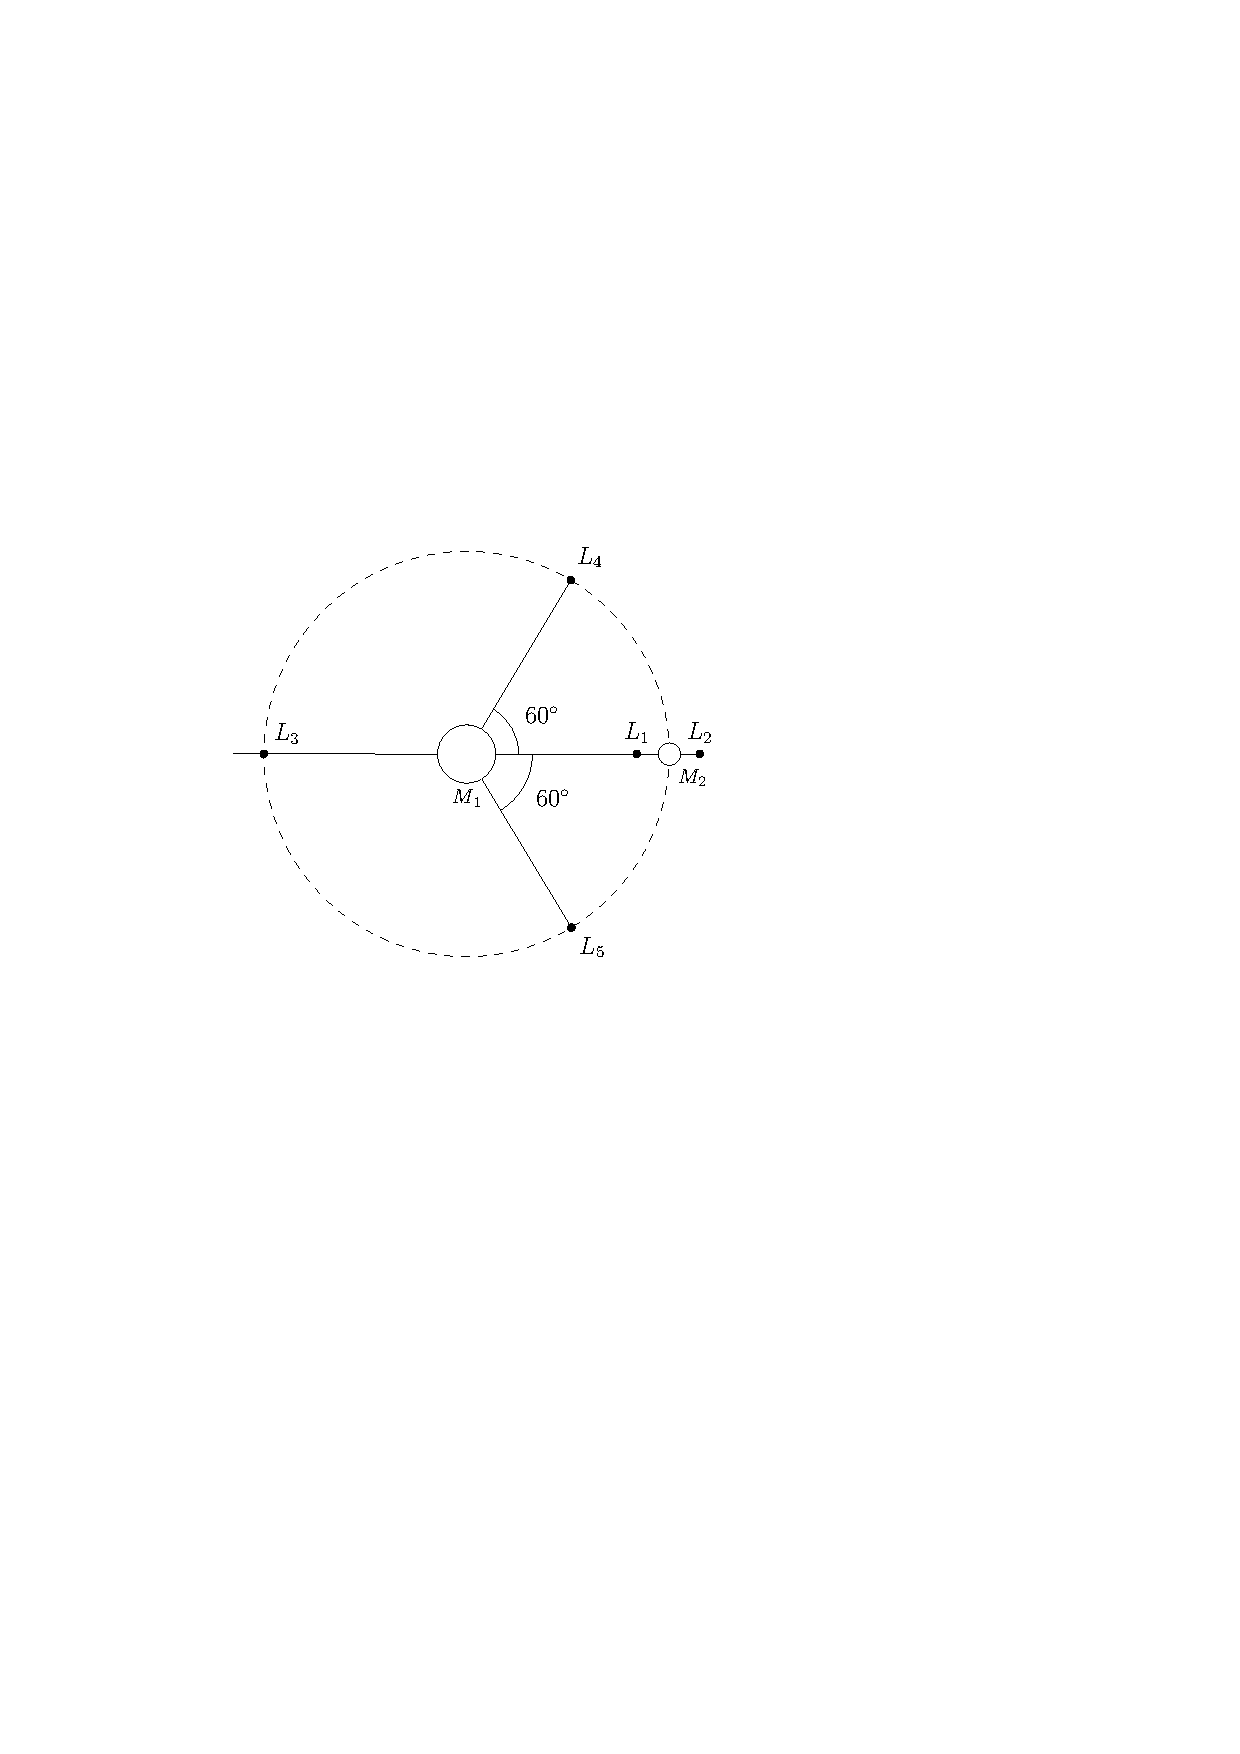
\includegraphics[width = 0.5\textwidth]{lagr-points}
\caption{Точки Лагранжа}\label{pic:lagr-points}
\end{figure}

Для расстояний до точек $L_1$, $L_2$ и $L_3$ от 
центра масс системы справедливы следующие выражения:
\begin{equation}r_1=R\left(1-\sqrt[3]{\frac{\alpha}
{3}}\right), \quad r_2=R\left(1+\sqrt[3]{\frac{\alpha}
{3}}\right), \quad r_3=\left(1+\frac{5}{12}\alpha\right),
\end{equation}
где $\alpha=M_1/(M_2+M_3)$, $R$ --- расстояние между 
телами, $M_1$ --- масса более массивного тела, $M_2$
 --- масса второго тела.

Если $M_2\ll M_1$, то точки $L_1$ и $L_2$ находятся 
примерно на равном расстоянии от тела $M_2$. 
Примерное значение этого расстояния определяется следующим 
выражением\begin{equation}
r\approx R\sqrt[3]{\frac{M_2}{3M_1}}
\end{equation}
